\documentclass[a0paper,portrait]{baposter}
\usepackage{biblatex}
\usepackage[font=small,labelfont=bf]{caption} % Required for specifying captions to tables and figures
\usepackage{booktabs} % Horizontal rules in tables
\usepackage{relsize} % Used for making text smaller in some places
\addbibresource{bib.bib}
\graphicspath{{figures/}} % Directory in which figures are stored

\definecolor{bordercol}{RGB}{40,40,40} % Border color of content boxes
\definecolor{headercol1}{RGB}{186,215,230} % Background color for the header in the content boxes (left side)
\definecolor{headercol2}{RGB}{80,80,80} % Background color for the header in the content boxes (right side)
\definecolor{headerfontcol}{RGB}{0,0,0} % Text color for the header text in the content boxes
\definecolor{boxcolor}{RGB}{186,215,230} % Background color for the content in the content boxes

\begin{document}

\background{ % Set the background to an image (background.pdf)
\begin{tikzpicture}[remember picture,overlay]
\draw (current page.north west)+(-2em,2em) node[anchor=north west]
{\includegraphics[height=1.1\textheight]{background}};
\end{tikzpicture}
}

\begin{poster}{
grid=false,
borderColor=bordercol, % Border color of content boxes
headerColorOne=headercol1, % Background color for the header in the content boxes (left side)
headerColorTwo=headercol2, % Background color for the header in the content boxes (right side)
headerFontColor=headerfontcol, % Text color for the header text in the content boxes
boxColorOne=boxcolor, % Background color for the content in the content boxes
headershape=roundedright, % Specify the rounded corner in the content box headers
headerfont=\Large\sf\bf, % Font modifiers for the text in the content box headers
textborder=rectangle,
background=user,
headerborder=open, % Change to closed for a line under the content box headers
boxshade=plain
}
{}
%
%----------------------------------------------------------------------------------------
%	TITLE AND AUTHOR NAME
%----------------------------------------------------------------------------------------
%
{\smaller Using Speech Recognition and Social Media to Diagnose Mental Illness} % Poster title
{\vspace{1em} Lynne Diep\\ % Author names
{\smaller Computer Science Department,
Jack Baskin School of Engineering\\
University of California, SantaCruz}}


%----------------------------------------------------------------------------------------
%	INTRODUCTION
%----------------------------------------------------------------------------------------

\headerbox{Introduction}{name=introduction,column=0,row=0}{

Using artificial intelligence in the medical field is no shock, but what if we use these same methods in diagnosing mental illness? Current algorithms in use are rated in their performance in the table below, and have helped doctors determine medical illness effectively. Surely the same contemplative process the machine goes through can help those in the psychiatric field. Here we will discuss the incorporation of artificial intelligence in a psychological setting. The results of this research will provide more insight on better determining mental illness to those who seek professional help in specific circumstances.

\begin{center}
\scalebox{0.4}{
 \begin{tabular}{||c c c c c c||} 
 \hline
 Classifier & Performance & Transparency & Explanation & Reduction & Missing data handling \\ [0.5ex] 
 \hline\hline
 Assistant-R & Good & Very good & Good & Good & Acceptable \\ 
 \hline
 Assistant-I & Good & Very good & Good & Good & Acceptable \\
 \hline
 LFC & Good & Good & Good & Good & Acceptable \\
 \hline
 Naive Bayes & Very good & Good & Very good & No & Very good \\
 \hline
 Semi-naive Bayes & Very good & Good & Very good & No & Very good \\ 
 \hline
 Backpropagation & Very good & Poor & Poor & No & Acceptable
 \\
 \hline
 $k$-NN & Very good & Poor & Acceptable & No & Acceptable\\ [1ex]
 \hline
\end{tabular}}
\end{center}
}

%----------------------------------------------------------------------------------------
%	MATERIALS AND METHODS
%----------------------------------------------------------------------------------------


%----------------------------------------------------------------------------------------
%	CONCLUSION
%----------------------------------------------------------------------------------------

\headerbox{Conclusion}{name=conclusion,column=0,below=introduction}{
\\
\begin{itemize}
    \item RNN is able to translate an output to a decoded transcription that displays proper sentences easier to read and understand.
    \item With SVM, the ability to analyze an image post's textual descriptions and "tags" the user has associated with is possible, and presents doctors more evidence when diagnosing a patient.
    \item Using features like color, texture, shape and SIFT when analyzing an image can uncover impactful data that would of otherwise been overlooked by human means.
    \item There is more research to be done in order for AI to successfully diagnose patients with mental illness. Important for AI to consider all types of mental illness and its various symptoms because not all cases are the same.
\end{itemize}
}

%----------------------------------------------------------------------------------------
%	REFERENCES
%----------------------------------------------------------------------------------------

\headerbox{References}{name=references,column=0,below=conclusion}{
\AtNextBibliography{\smaller}
\printbibliography[heading=none]

}


\headerbox{Contact Details}{name=contact,column=0,below=references}{
\begin{center}
Lynne Diep\\
University of California, Santa Cruz\\
Email: lytdiep@ucsc.edu\\
Phone: (345)234-4567 \\
\hfill \break
\hfill \break

\includegraphics[scale=0.5]{logo}\\
\hfill \break
\end{center}

}
%----------------------------------------------------------------------------------------
%	RESULTS 1
%----------------------------------------------------------------------------------------

\headerbox{Speech Recognition}{name=results1,span=2,column=1,row=0}{ % To reduce this block to 1 column width, remove 'span=2'
\begin{itemize}
    \item The core of a speech recognition system is a Recurrent Neural Network, or RNN trained to ingest speech spectrograms and generate English text transcriptions.
    \item Each utterance a user makes is a vector of audio features.
    \item Spectrograms will act as the features, which denote the power of the frequency bin in the audio frame at time.
    \item The goal of our RNN is to convert an input sequence into a sequence of character probabilities for the transcription.
    \item RNN algorithm can learn to generate readable character-level transcriptions.
\end{itemize}
The results of this algorithm is satisfactory, as it transcribes the input into a readable, define output. In the table below, an example of transcription is given. \cite{DBLP:journals/corr/HannunCCCDEPSSCN14}



%------------------------------------------------

\begin{center}
\begin{tabular}{l l}
\toprule
\textbf{RNN Output} & \textbf{Decoded Transcription}\\
\midrule
what is the weather like in bostin right now & what is the weather like in boston right now \\
prime miniter & prime minister \\
arther n tikets for the game & are there any tickets for the game   \\
\bottomrule
\end{tabular}
\captionof{table}{Transcription Example}
\end{center}
}

%----------------------------------------------------------------------------------------
%	RESULTS 2
%----------------------------------------------------------------------------------------

\headerbox{Text and Image Analysis on Social Media}{name=results2,span=2,column=1,below=results1,above=bottom}{ % To reduce this block to 1 column width, remove 'span=2'
\begin{itemize}
    \item Support Vector Machine, or SVM is a part of machine learning and is used to analyze textual descriptions and classify them using predetermined set of terms.
    \item Phrases will be analyzed and specific weights will be added to them to determine the significance.
    \item As each word in the patient's phrase is analyzed and assigned weights, the total weight is a part of a determining factor in a psychiatrist's diagnosis.
    \item The correlation between text analysis and actual health statistics is not inaccurate either, so it does provide stable evidence when diagnosing an individual as seen in Figure 1.\cite{Sadilek:2013:MIL:2433396.2433476}
\end{itemize}

%------------------------------------------------

\begin{center}
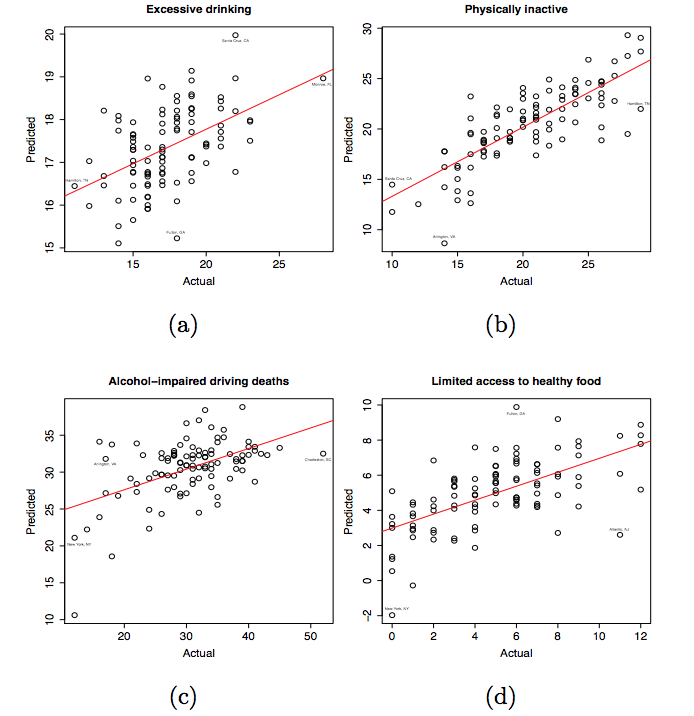
\includegraphics[width=200px]{Figure1}
\captionof{figure}{Predicted vs.\hspace{1mm}actual health statistics value}
\end{center}

%------------------------------------------------
\\
\\
\begin{itemize}
    \item Using features like color, texture, shape and Scale Invariant Feature Transform (SIFT) when analyzing an image can uncover impactful data that would of otherwise been overlooked by human means.
    \item Image analysis is able to pinpoint specific shapes within the image, like a syringe or bottle.
    \item Texture is another strong feature; users are able to edit their photos and change the tone of it, as some filters correlate with mental illness as seen in Figure 2.\cite{5202725}
\end{itemize}

\begin{center}
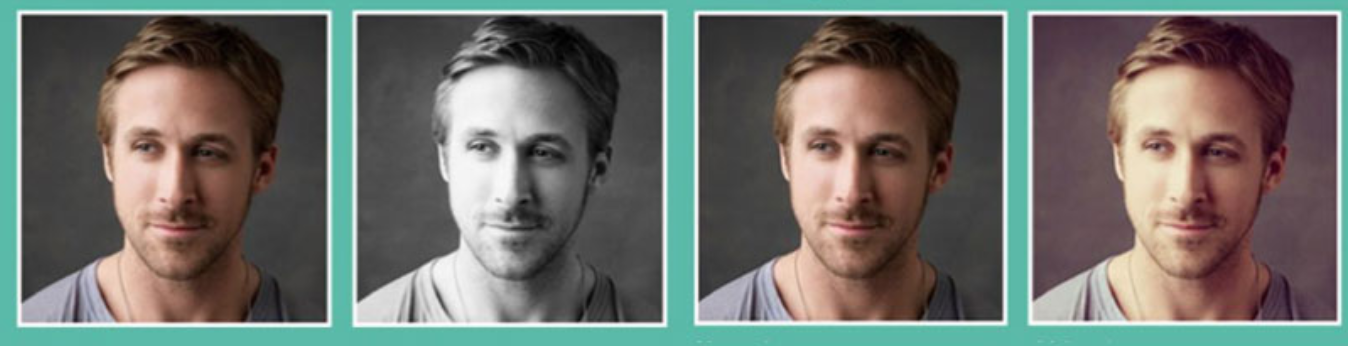
\includegraphics[width=0.49\linewidth]{Figure2}
\captionof{figure}{Inkwell - correlates with depression (left); Valencia - most likely used by healthy individuals(right)}
\end{center}
}
\hfill \break 
\end{poster}

\end{document}